\documentclass[a4paper]{article}

\usepackage{fullpage} % Package to use full page
\usepackage{parskip} % Package to tweak paragraph skipping
\usepackage{tikz} % Package for drawing
\usepackage{amsmath}
\usepackage{hyperref}

\title{Understanding the Derivative}
\author{Vincent Knight}
\date{1984/02/14}

\begin{document}

\maketitle

\section{Introduction}

Differentiation is a concept of Mathematics studied in Calculus. There is an ongoing discussion as to who was the first to define differentiation: Leibniz or Newton \cite{bardi2006calculus}.

Differentiation allows for the calculation of the slope of the tangent of a curve at any given point as shown in Figure \ref{exampleplot}.

\begin{figure}[!htbp]
\begin{center}
\begin{tikzpicture}
\draw[domain=-2:2, color=blue] plot (\x, {1 - (\x)^2}) node[above = .5cm, right, color=blue] {$f(x)=1-x^2$};
\draw[domain=-2:2, color=red] plot(\x,-1 * \x + 1.25) node[above = .5cm, right, color=red] {Tangent at $x=.5$};
\draw [thick, ->] (-3,0) -- (3,0) node [above] {$x$};
\draw [thick, ->] (0,-3) -- (0,3) node [right] {$y$};
\node at (.5,.75) {\textbullet};
\end{tikzpicture}
\end{center}
\caption{The plot of $f(x)=1-x^2$ with a tangent at $x=.5$.}\label{exampleplot}
\end{figure}

Differentiation is now a technique taught to mathematics students throughout the world. In this document I will discuss some aspects of differentiation.

\section{Exploring the derivative using Sage}

The definition of the limit of $f(x)$ at $x=a$ denoted as $f'(a)$ is:

\begin{equation}
f'(a) = \lim_{h\to0}\frac{f(a+h)-f(a)}{h}
\end{equation}

The following code can be used in sage to give the above limit:

\begin{verbatim}
def illustrate(f, a):
    """
    Function to take a function and illustrate the limiting definition of a derivative at a given point.
    """
    lst = []
    for h in srange(.01, 3, .01):
    	lst.append([h,(f(a+h)-f(a))/h])
    return list_plot(lst, axes_labels=['$x$','$\\frac{f(%.02f+h)-f(%.02f)}{h}$' % (a,a)])
\end{verbatim}

\begin{figure}[!htbp]
\begin{center}
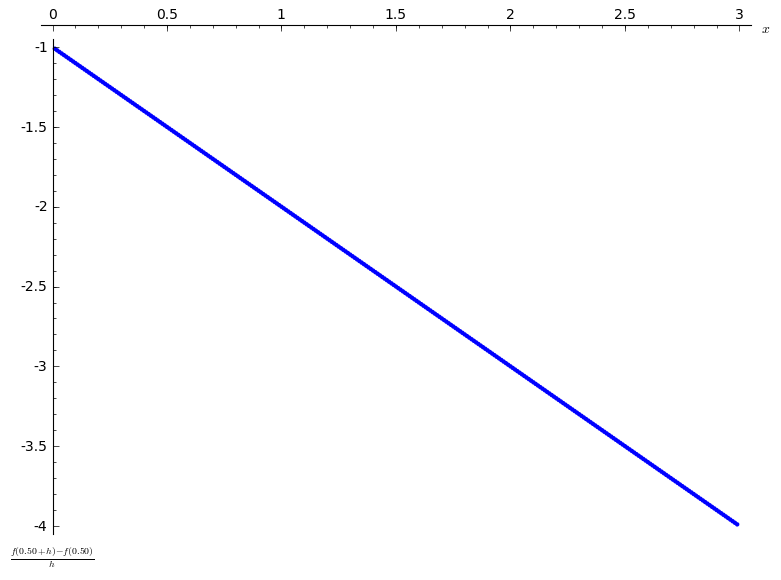
\includegraphics[width=8cm]{sage1.png}
\end{center}
\caption{The derivative of $f(x)=1-x^2$ at $x=.5$ converging to -1 as $h\to0$.}
\end{figure}

If we want to plot the tangent at a point $\alpha$ to a function we can use the following:

\begin{align}
y=&ax+b&&\text{(definition of a straight line)}\nonumber\\
  &f'(a)x+b&&\text{(definition of the derivative)}\nonumber\\
  &f'(a)x+f(a)-f'(a)a&&\text{(we know that the line intersects $f$ at $(a,f(a))$}\nonumber
\end{align}

We can combine this with the approach of the previous piece of code to see how the tangential line converges as the limiting definition of the derivative converges:

\begin{verbatim}
def convergetangentialline(f, a, x1, x2, nbrofplots=50, epsilon=.1):
    """
    Function to make a tangential line converge
    """
    clrs = rainbow(nbrofplots)
    k = 0
    h = epsilon
    p = plot(f, x, x1, x2)
    while k < nbrofplots:
        tangent(x) = fdash(f, a, h) * x + f(a) - fdash(f, a, h) * a
        p += plot(tangent(x), x, x1, x2, color=clrs[k])
        h += epsilon
        k += 1
    return p
\end{verbatim}

The plot shown in Figure \ref{lines} shows how the lines shown converge to the actual tangent to $1-x^2$ as $x=2$ (the red line is the `closest' curve).

\begin{figure}[!htbp]
\begin{center}
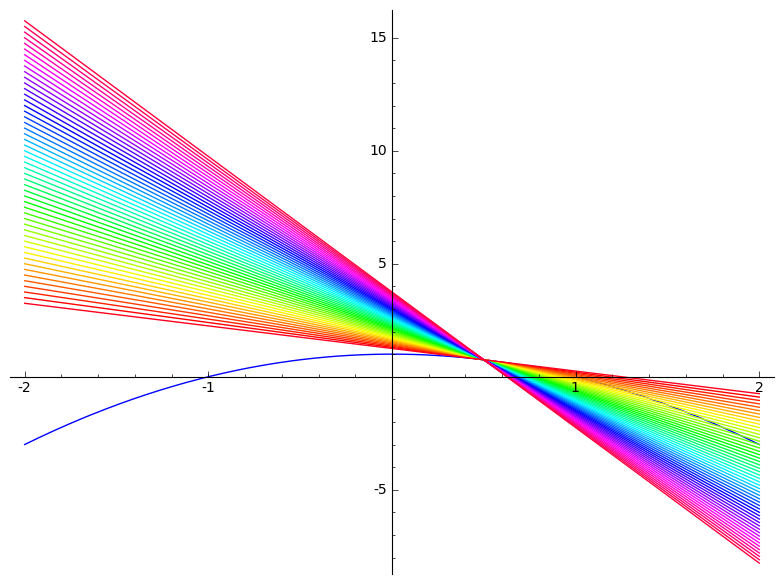
\includegraphics[width=8cm]{sage0.png}
\end{center}
\caption{Lines converging to the tangent curve as $h\to0$.}\label{lines}
\end{figure}

Note here that the last plot is given using the \textbf{real} definition of the derivative and not the approximation.

\section{Conclusions}

In this report I have explored the limiting definition of the limit showing how as $h\to 0$ we can visualise the derivative of a function. The code involved \url{https://sage.maths.cf.ac.uk/home/pub/18/} uses the differentiation capabilities of Sage but also the plotting abilities.

There are various other aspects that could be explored such as symbolic differentiation rules. For example:

$$\frac{dx^n}{dx}=(n+1)x^{n}\text{ if }x\ne-1$$

Furthermore it is interesting to not that there exists some functions that \textbf{are not} differentiable at a point such as the function $f(x)=\sin(1/x)$ which is not differentiable at $x=0$. A plot of this function is shown in Figure \ref{notdiff}.

\begin{figure}[!htbp]
\begin{center}
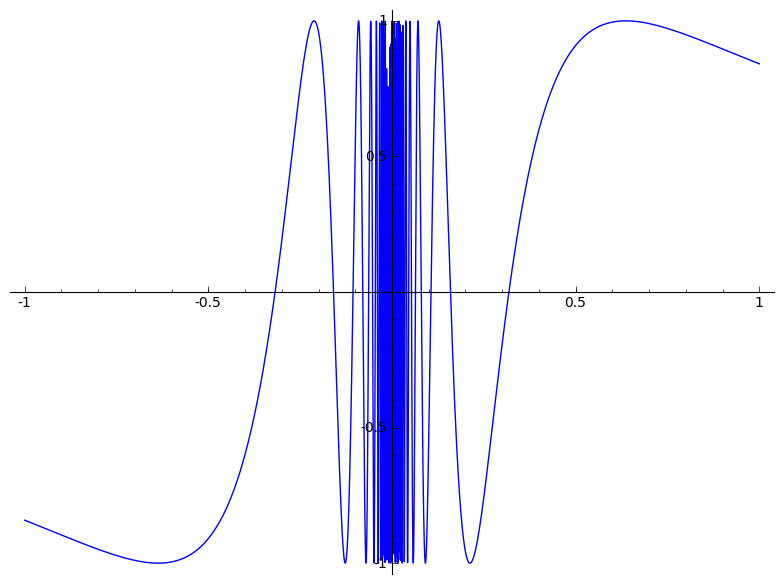
\includegraphics[width=8cm]{sage2.png}
\end{center}
\caption{None differentiable function at $x=0$.}\label{notdiff}
\end{figure}


\bibliographystyle{plain}
\bibliography{bibliography.bib}
\end{document}